\documentclass[handout]{beamer}

\usepackage{Haust2017glærur}

\title{Stærðfræðimynstur í tölvunarfræði}
\subtitle{Vika 11, fyrri fyrirlestur}

\begin{document}

\begin{frame}
\titlepage
\end{frame}


\section{Inngangur}

\begin{frame}{Í síðasta tíma}
\begin{itemize}
 \item Kosningareiknirit
 \item Nokkrar gerðir sérstakra neta
 \item Spyrðingar
 \item Framsetning á netum
\end{itemize}
\end{frame}

\section{Vegur í neti}

\begin{frame}{Vegur í neti}
Skilgreining á vegi (e.  path) kemur víða við í netafræði.

\begin{tcolorbox}[title=Vegur]
Látum $n$ vera ekki-neikvæða heiltölu. Þá er vegur af lengd $n$ frá hnúti $u$ í $G$ til hnúts $v$ í $G$ runa $e_1, \ldots, e_n$ af leggjum í $G$ sem hefur þann eiginleika að til sé runa $x_0 = u, x_1, \ldots, x_{n-1}, x_n = v$ af hnútum í $G$ svo að fyrir öll $i = 1, \ldots, n$, hafi leggurinn $e_i$ endahnútana $x_{i-1}$ og $x_i$.
\end{tcolorbox}
\end{frame}

\begin{frame}{Um vegi}
\begin{itemize}
 \item Veg þar sem allir leggirnir eru aðskildir má kalla einfaldan (e. \emph{simple})
 \item Veg af jákvæðri lengd þar sem upphafs- og endahnúturinn er sami hnútur má kalla rás (e. \emph{circuit})
 \item Þegar um er að ræða einfalt net getum við táknað veg með því að telja upp hnútana sem hann snertir
 \item Í stefndu neti getum við á mjög svipaðan hátt skilgreint stefnda vegi/örvavegi (e. \emph{directed paths})
 \item Athugum vandlega: Mismunandi skilgreiningar eru til á vegum og einföldum vegum, þetta er skilgreiningin sem bókin notar
\end{itemize}
\end{frame}

\begin{frame}{Vegir í samfélagsneti}
\begin{center}
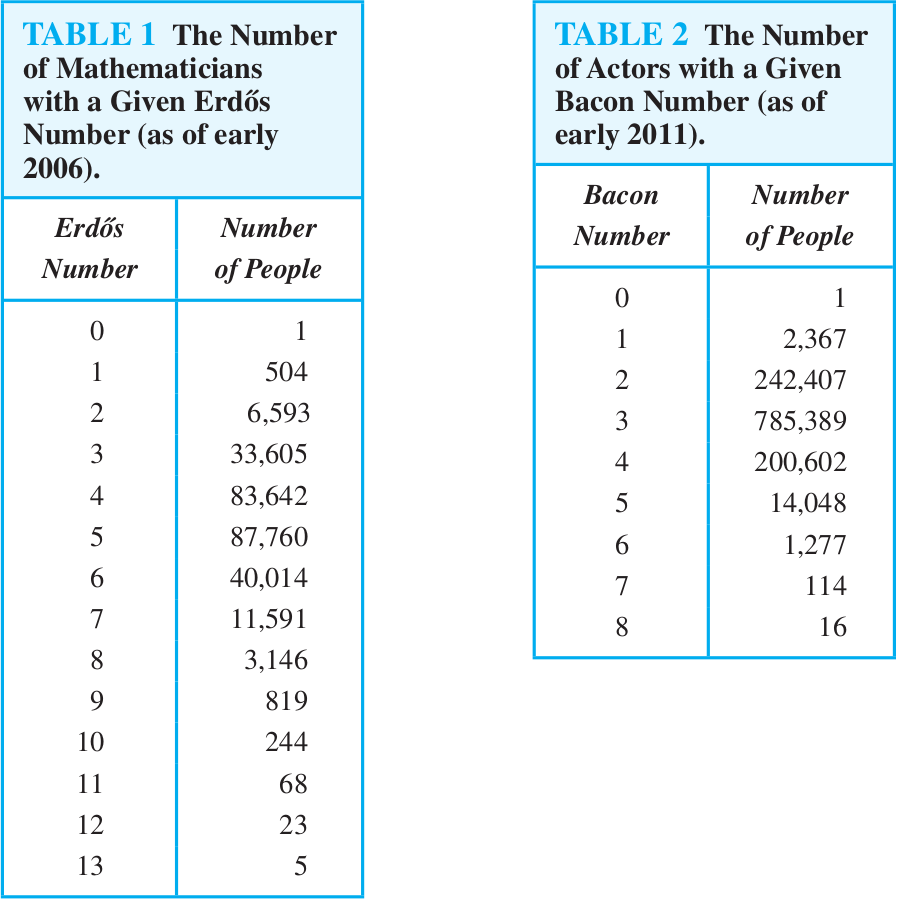
\includegraphics[width=0.7\textwidth]{path-length}
\end{center}
\end{frame}

\section{Samhengi og samhengisþættir}

\begin{frame}{Samanhangandi net}
Út frá skilgreiningu á vegi fáum við skilgreiningu á samanhangandi (e. \emph{connected}) neti:
\begin{tcolorbox}[title=Samanhangandi net]
Óstefnt net er kallað samanhangandi sé til vegur á milli hverra tveggja aðskildra hnúta í netinu.
\end{tcolorbox}
Af henni má leiða setningu:
\begin{tcolorbox}
Til er einfaldur vegur á milli hverra tveggja aðskildra hnúta í óstefndu samanhangandi neti.
\end{tcolorbox}

\end{frame}

\begin{frame}{Samhengisþættir}
Út frá skilgreiningu á hlutmengi getum við skilgreint hlutnet:
\begin{tcolorbox}[title=Hlutnet]
Hlutnet nets $G$ er net $H$ sem hefur þá eiginleika að hnútamengi $H$ er hlutmengi hnútamengis $G$ og leggjamengi $H$ er hlutmengi leggjamengis $G$.
\end{tcolorbox}
\pause
Getum þá skilgreint samhengisþátt:
\begin{tcolorbox}
Samhengisþáttur (e. \emph{connected component}) nets $G$ er hlutnet $G$ sem er samanhangandi og óstækkanlegt sem slíkt.
\end{tcolorbox}
Ósamanhangandi net hefur meira en einn samhengisþátt.
\end{frame}

\begin{frame}{Þrjú net}
\begin{center}
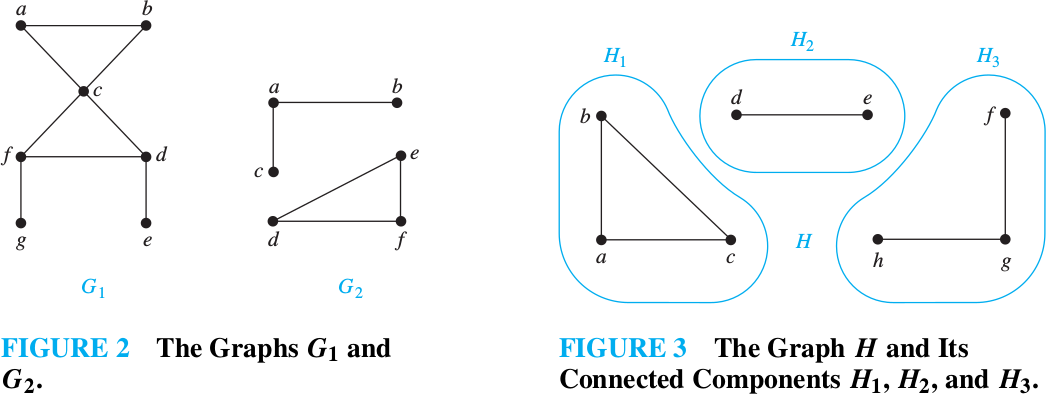
\includegraphics[width=\textwidth]{graph-connectivity}
\end{center}
\end{frame}

\begin{frame}{Brýr}
\begin{tcolorbox}[title=Brú]
Leggur $e$ í $G$ kallast brú (e. \emph{bridge} eða \emph{cut edge}) ef hlutnetið sem myndað er með því að fjarlægja $e$ úr $G$ hefur fleiri samhengisþætti en $G$.
\end{tcolorbox}
Svipaða skilgreiningu má setja fram fyrir hnúta. Slíkir hnútar eru kallaðir ``cut vertices'' í bókinni.
\end{frame}

\begin{frame}{Bandaríska þingið}
    \begin{center}
        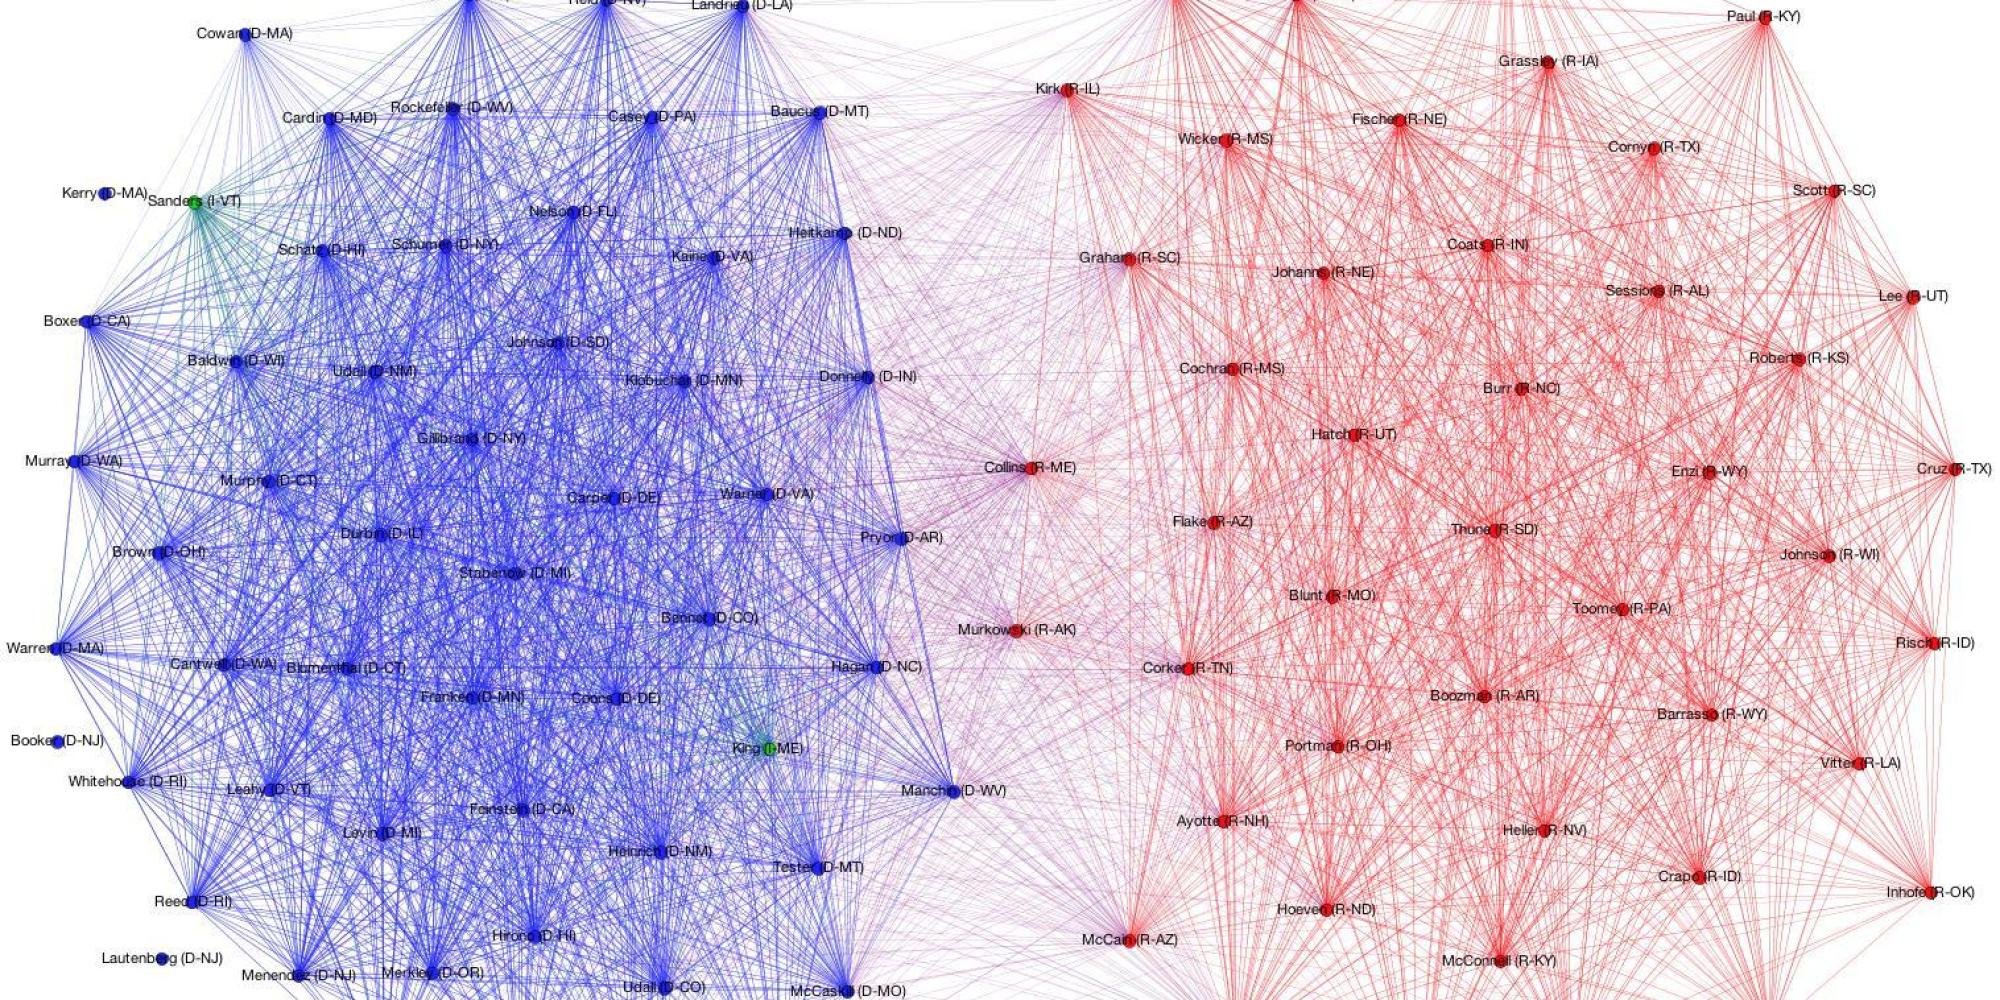
\includegraphics[width=\textwidth]{polarization}
    \end{center}
\end{frame}

\begin{frame}{Samhengi}
Við getum skilgreint hnútasamhengi (e. \emph{vertex connectivity}) nets.

\begin{tcolorbox}[title=Samhengi]
Talan $\kappa(G)$ táknar hnútasamhengi netsins $G$. $\kappa(G)$ er lágmarksfjöldi hnúta sem þarf að fjarlægja úr $G$ til að mynda net sem er ósamanhangandi eða með einungis einn hnút.
\end{tcolorbox}
Ósamanhangandi net er með $\kappa(G) = 0$. $\kappa(K_n) = n-1$.
\end{frame}

\begin{frame}{Samhengi og örvanet}
\begin{tcolorbox}[title=Stranglega samanhangandi örvanet]
Örvanet er stranglega samanhangandi (e. \emph{strongly connected}) ef til er örvavegur frá $a$ til $b$ og frá $b$ til $a$ fyrir sérhverja hnúta $a$ og $b$ í örvanetinu.
\end{tcolorbox}

\begin{tcolorbox}[title=Veikt samanhangandi örvanet]
Örvanet er veikt samanhangandi (e. \emph{weakly connected}) sé tilsvarandi óstefnt net samanhangandi.
\end{tcolorbox}
\end{frame}

\begin{frame}{Samanhangandi örvanet}
\begin{center}
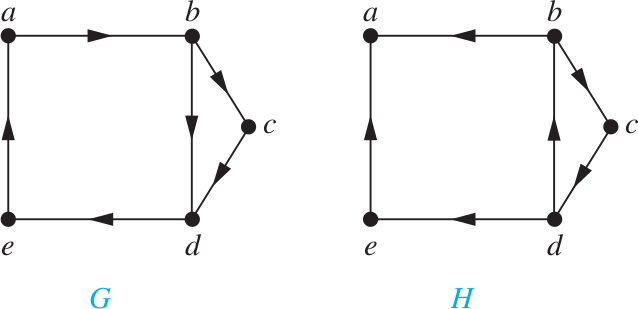
\includegraphics[width=\textwidth]{graph-strong-weak-connected}
\end{center}
\end{frame}
\section{Fjöldi vega}
\begin{frame}{Fjöldi vega}
\begin{tcolorbox}
Látum $G$ vera net með grennslafylkið $A$ m.t.t. hnútaröðunar $v_1, \ldots, v_n$. Þá er fjöldi mismunandi vega af jákvæðri lengd $r$ á milli hnúta $v_i$ og $v_j$ talan sem er í sæti $i,j$ í fylkinu $A^r$.
\end{tcolorbox}
\end{frame}

\begin{frame}{Dæmi}
Finnum fjölda mismunandi vega á milli $a$ og $d$ í eftirfarandi neti:
\begin{columns}
\column{0.25\textwidth}
\begin{center}
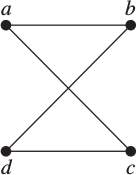
\includegraphics[width=\linewidth]{graph-mini}
\end{center}
\column{0.75\textwidth}
\[
A =
\begin{bmatrix}
0&1&1&0\\
1&0&0&1\\
1&0&0&1\\
0&1&1&0\\
\end{bmatrix}
,
A^4 =
\begin{bmatrix}
8&0&0&8\\
0&8&8&0\\
0&8&8&0\\
8&0&0&8\\
\end{bmatrix}
\]
\begin{center}
Svo fjöldi veganna er 8.
\end{center}
\end{columns}
\end{frame}

\section{Euler-vegir}

\begin{frame}{Elsta netavandamálið}
Í borginni Königsberg voru eitt sinn 7 brýr.
\begin{center}
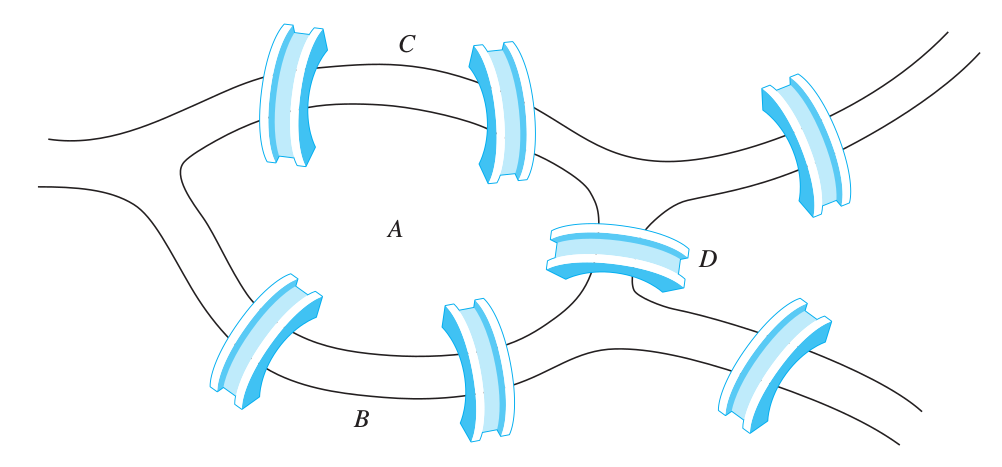
\includegraphics[width=0.8\textwidth]{konigsberg}
\end{center}
Er hægt að fara í göngutúr sem endar á sama stað og hann byrjar og liggur yfir hverja brú nákvæmlega einu sinni?
\end{frame}

\begin{frame}{Netaframsetning}
\begin{columns}
\column{0.6\textwidth}
Stærðfræðingurinn Leonhard Euler leysti vandamálið með netaframsetningu.

Við getum skilgreint Euler-rás:

\begin{tcolorbox}[title=Euler-rás]
Euler-rás (e. \emph{Euler circuit}) í óstefndu neti $G$ er einföld rás sem inniheldur alla leggi í $G$.
\end{tcolorbox}
Er til Euler-rás í Königsberg-netinu?
\column{0.4\textwidth}
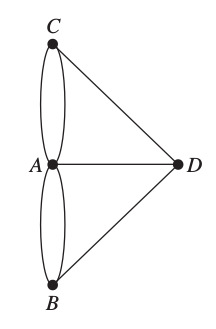
\includegraphics[width=\textwidth]{konigsberg-graph}
\end{columns}
\end{frame}

\begin{frame}{Euler-rásir}
Við getum fundið skilyrði sem er nauðsynlegt og nægjanlegt fyrir tilvist Euler-rásar í óstefndu neti.

\begin{tcolorbox}
Samanhangandi óstefnt net með a.m.k. tveimur hnútum hefur Euler-rás ef og aðeins ef stig allra hnúta í netinu er slétt tala.
\end{tcolorbox}

Königsberg-göngutúrinn okkar er þá ekki mögulegur.
\end{frame}

\begin{frame}{Dæmi}
Við getum fundið Euler-rás í þessu neti.
\begin{center}
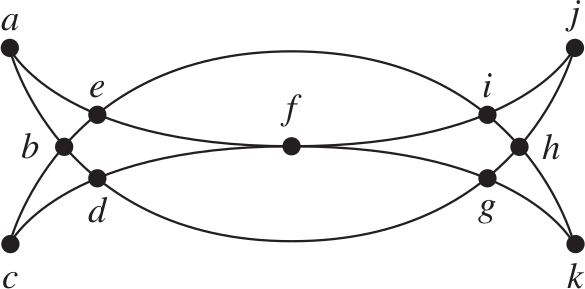
\includegraphics[width=0.6\textwidth]{mohammed-scimitars}
\end{center}
\pause
Möguleg lausn:
\[
a, b, d, g, h, j, i, h, k, g, f, d, c, b, e, i, f, e, a
\]

\end{frame}

\begin{frame}{Euler-vegir}
\begin{tcolorbox}[title=Euler-vegur]
Euler-vegur (e. \emph{Euler path}) í óstefndu neti $G$ er einfaldur vegur sem inniheldur alla leggi í $G$.
\end{tcolorbox}

\begin{tcolorbox}
Samanhangandi óstefnt net hefur Euler-veg og ekki Euler-rás ef og aðeins ef stig nákvæmlega tveggja hnúta í netinu er oddatala.
\end{tcolorbox}
\end{frame}

\begin{frame}{Hamilton- vegir og rásir}
    \begin{tcolorbox}[title=Hamilton-vegir og rásir]
    Einfaldur vegur í óstefndu neti sem fer í gegnum hvern hnút nákvæmlega einu sinni er kallaður Hamilton-vegur (e. \emph{Hamilton path}). Einföld rás sem fer nákvæmlega einu sinni í gegnum hvern hnút netsins er kölluð Hamilton-rás (e. \emph{Hamilton circuit}).
    \end{tcolorbox}
    Leit að Hamilton-vegum reynist vera miklu erfiðara vandamál!
\end{frame}

\begin{frame}{Næst}
Næst: Hamilton-vegir (10.5), vegin net og stystu vegir (10.6).

Þarnæst: Lagnet (10.7) og litun neta (10.8)
\end{frame}

\end{document}
